
\subsection{Overview}
The architecture of the system is composed of two main components: the \ac{eMSP} and the \ac{CPMS}.

\subsubsection{\ac{eMSP} overview}

\begin{figure}[!h]
    \begin{center}
        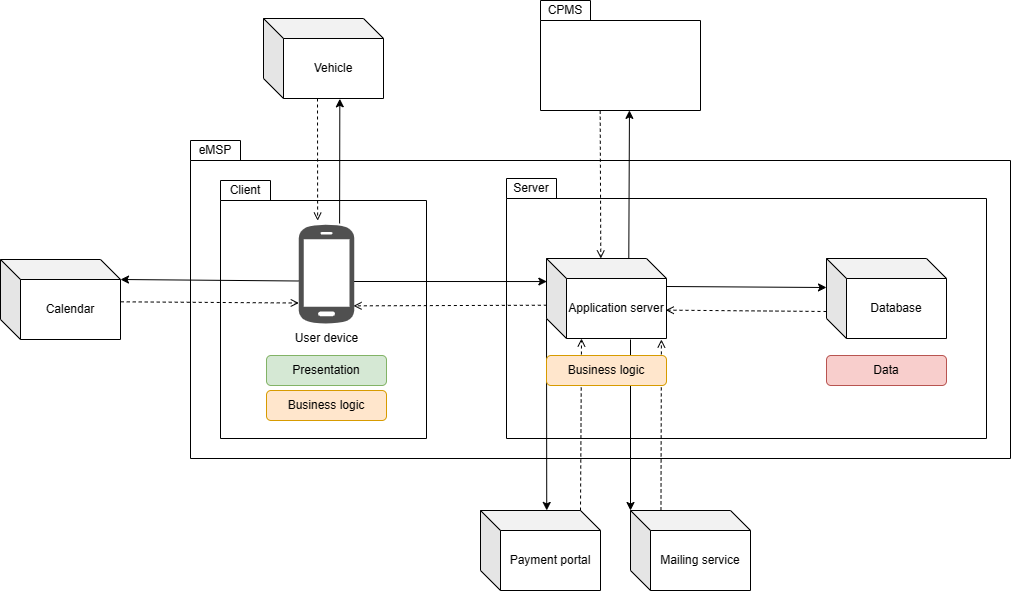
\includegraphics[keepaspectratio, width=0.75\textwidth]{Graphics/DD-eMSP-overview.drawio.png}
        \caption{\ac{eMSP} architectural overview}
        \label{fig:eMSP-overview-architecture}
    \end{center}
\end{figure}

The \ac{eMSP} is a \textbf{three-tier} architecture with \textbf{fat-clients} as seen in \autoref{fig:eMSP-overview-architecture}. This architecture is chosen for different reasons:
\begin{itemize}
    \item Makes the system more scalable;
    \item Allows the separation between business logic and data so that we can apply different levels of dependability to different decoupled systems and we can manage how data is accessed in a more granular way;
    \item There will be a lot of data to be handled in this system (such as booked charges, all the infos about \acp{CPO}, etc.); for this, a dedicated and optimized infrastructure is chosen to be the best choice;
    \item The database will only be accessible by the middleware, constituting an additional layer of security;
    \item With fat-clients the number of messages transmitted are fewer and lighter: an initial elaboration can be done on the smart devices of the user without sending a lot of raw data to the remote application server. The local on-the-edge elaboration is not considered as a problem given the computational power of smartphones.
\end{itemize}
The software pattern applied for this architecture will be the \textbf{\ac{MVC} pattern}. This is the best suit for our application because, being it a web application, we want the components to be as modular, flexible and scalable as possible in order to simplify their distribution.

The following paragraphs will describe the principal components of this pattern and their architectural distribution.

\paragraph{Model}
The model is the logical representation of the persistent data. This is stored in a database system and will only be directly accessible by the server application.

\paragraph{View}
The view logic will be completely delegated to the client application, representing in different ways the data retrieved from the model (e.g. the charging stations sorting based on the user selected preferences).

\paragraph{Controller}
The controller will have to manage all the client requests, interacting with the model, modifying it and returning to the view the changed/retrieved data.
In our application, for the most part, the business logic will be in the server application. Just the part of retrieving and processing the vehicle data the calendar appointments (in the case of a request for smart suggestions of the application) will be handled by the client application so that the communication with the application server will be as simple as possible.

\subsubsection{\ac{CPMS} overview}

\begin{figure}[!h]
    \begin{center}
        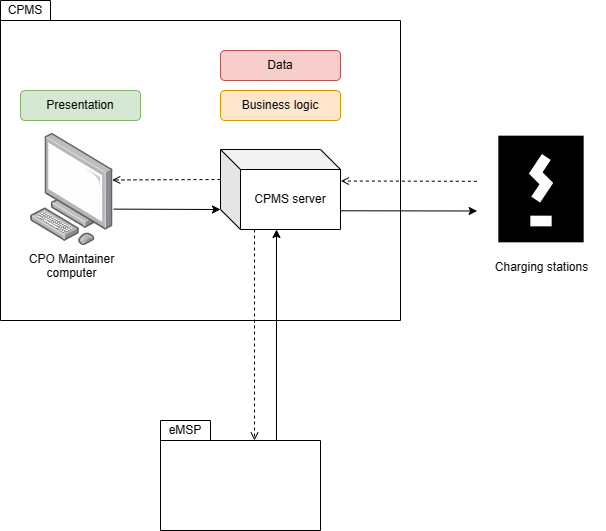
\includegraphics[keepaspectratio, width=0.75\textwidth]{Graphics/DD-CPMS-overview.drawio.png}
        \caption{\ac{CPMS} architectural overview}
        \label{fig:CPMS-overview-architecture}
    \end{center}
\end{figure}

The \ac{CPMS} follows the \textbf{two-tier} pattern with \textbf{thin-clients} as seen in \autoref{fig:CPMS-overview-architecture}. This architecture is chosen for different reasons:
\begin{itemize}
    \item The system is simpler to implement with respect to the three-tier architecture;
    \item The system shouldn't handle so much data, so it isn't necessary to have a dedicated architecture for the data layer;
    \item Clients are thin because they only have to view infos about charging stations and can send simple events (for example \textit{use \ac{DSO} X for charging station Y}, \textit{set revenue percentage to Z}, etc.).
\end{itemize}
Also for this system we will use the \ac{MVC} pattern. In this case, the client will only have the view logic and can send simple events. All the elaboration, the management of the \acp{DSO} and activation/deactivation of charging process of batteries are handled by the \ac{CPMS} server, which handles the business logic and the data.
The \ac{CPMS} server, on the other hand, will deal also with charging requests from \acp{eMSP}, to which it will respond with the elaborated data.


\subsection{Component view}
\begin{figure}[!h]
    \begin{center}
        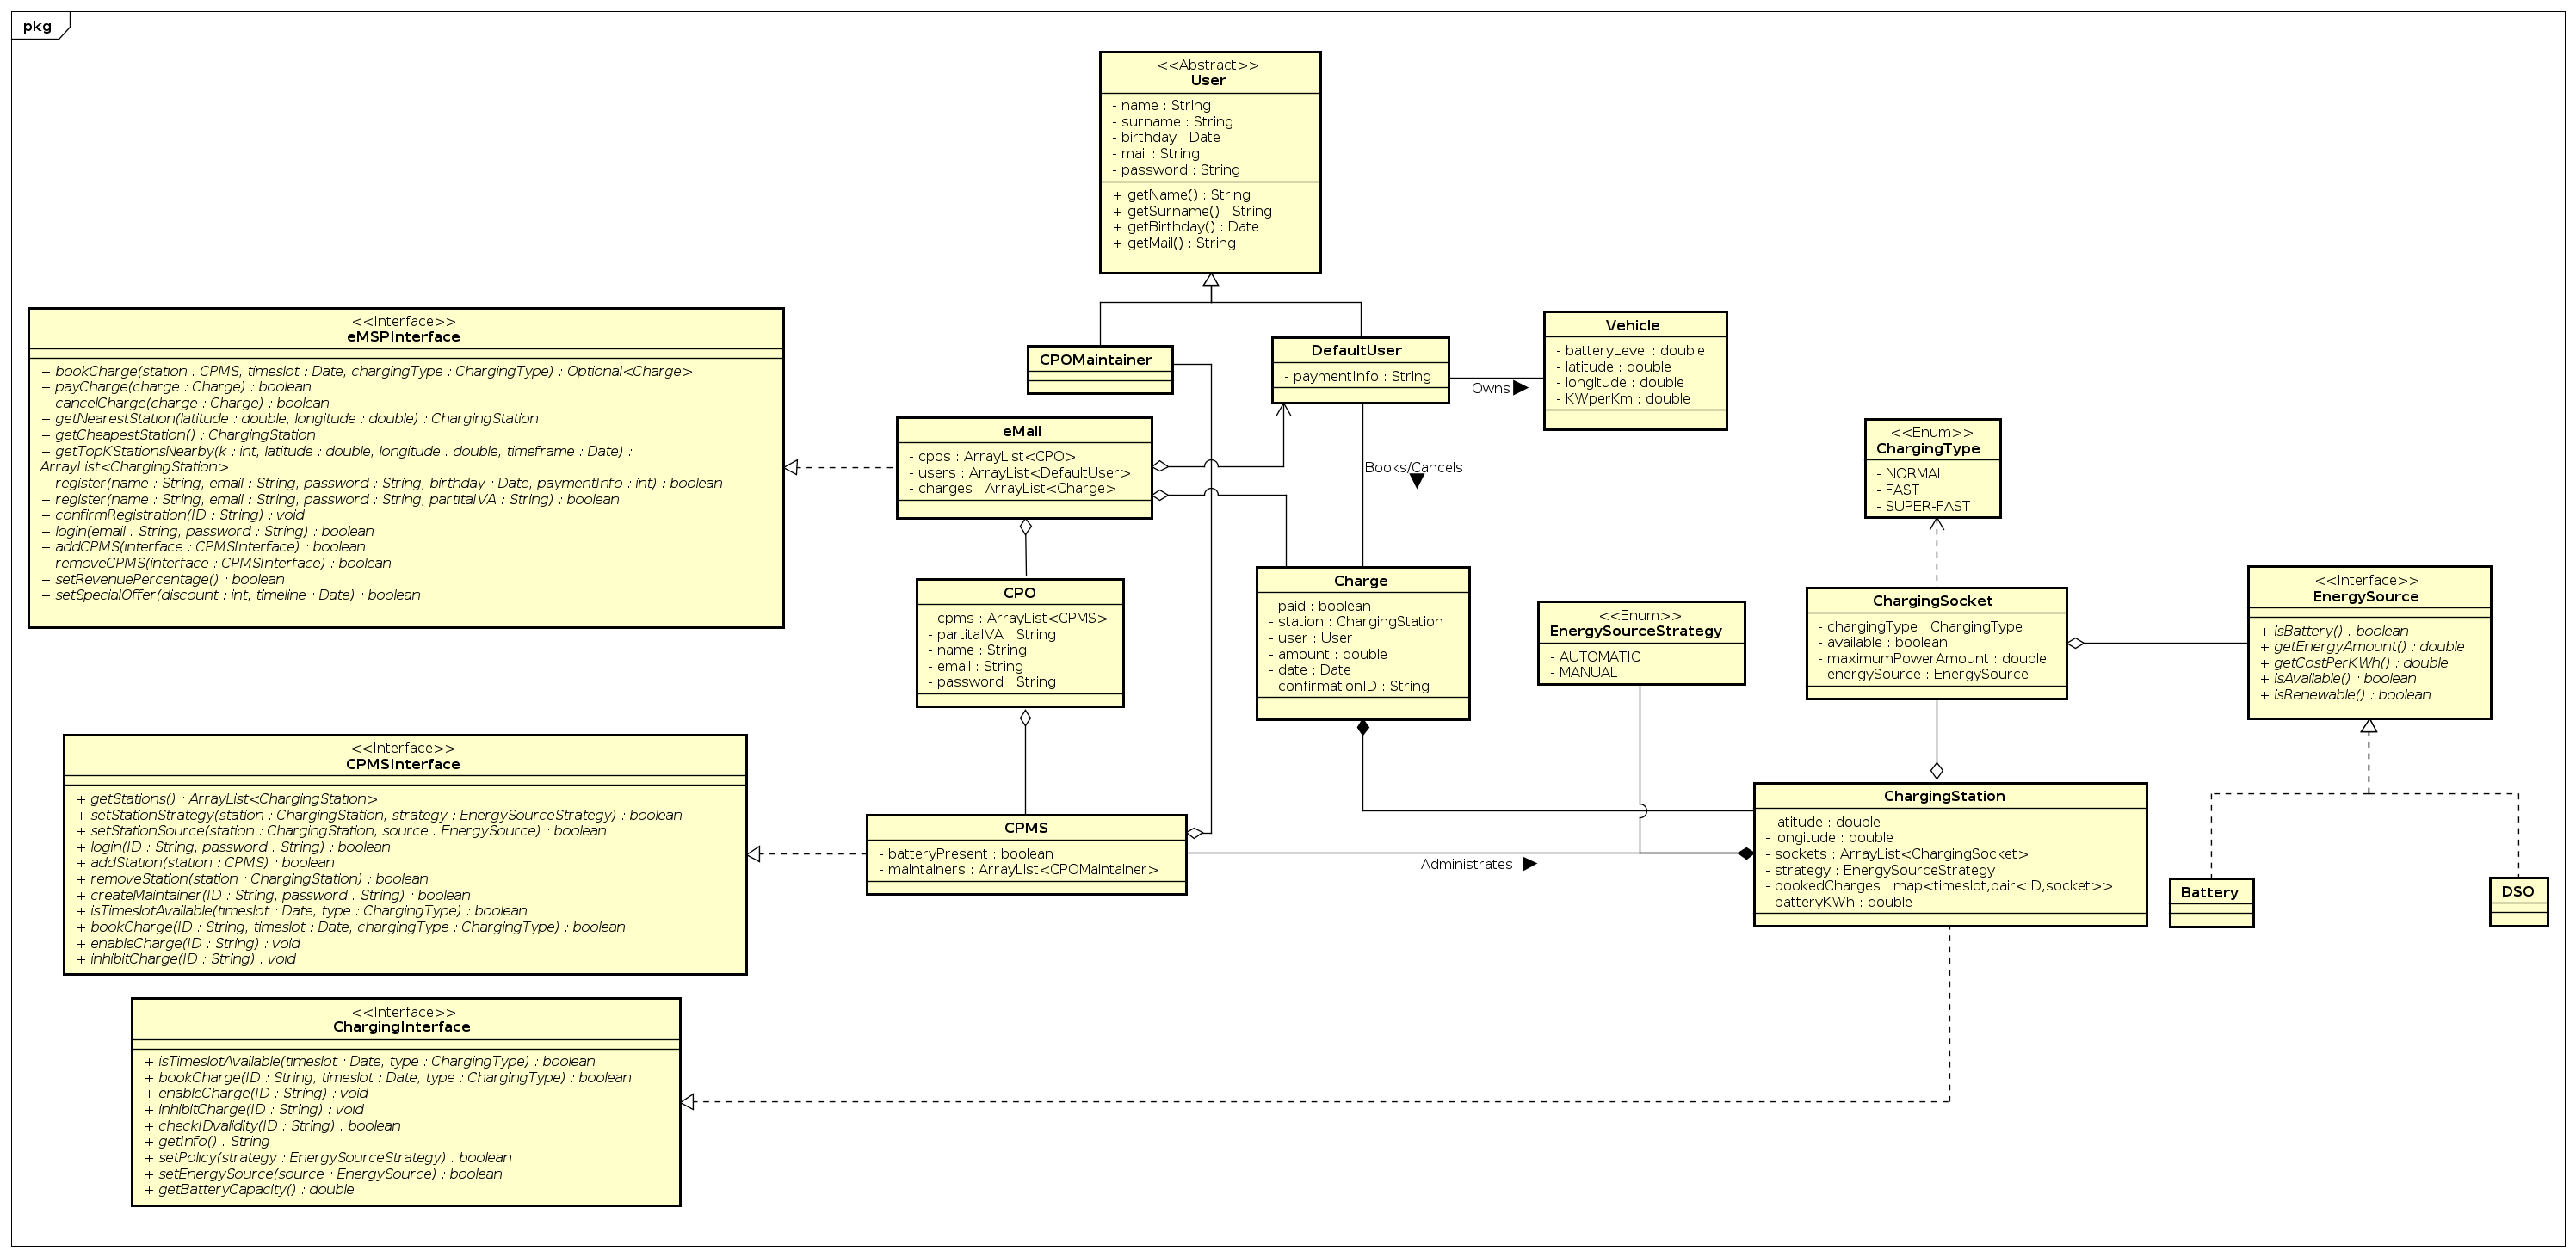
\includegraphics[keepaspectratio, width=16cm]{UML.png}
        \caption{Class diagram}
        \label{fig:UML}
    \end{center}
\end{figure}
In the class diagram illustrated in \autoref{fig:UML} a model (not functional) view of the system is represented. The \ac{eMall} and \ac{CPMS} interfaces show what the two systems are expected to implement, whereas for the ChargingInterface it is assumed an already existing implementation.

\subsubsection{Component diagrams}
\begin{figure}[!h]
    \begin{center}
        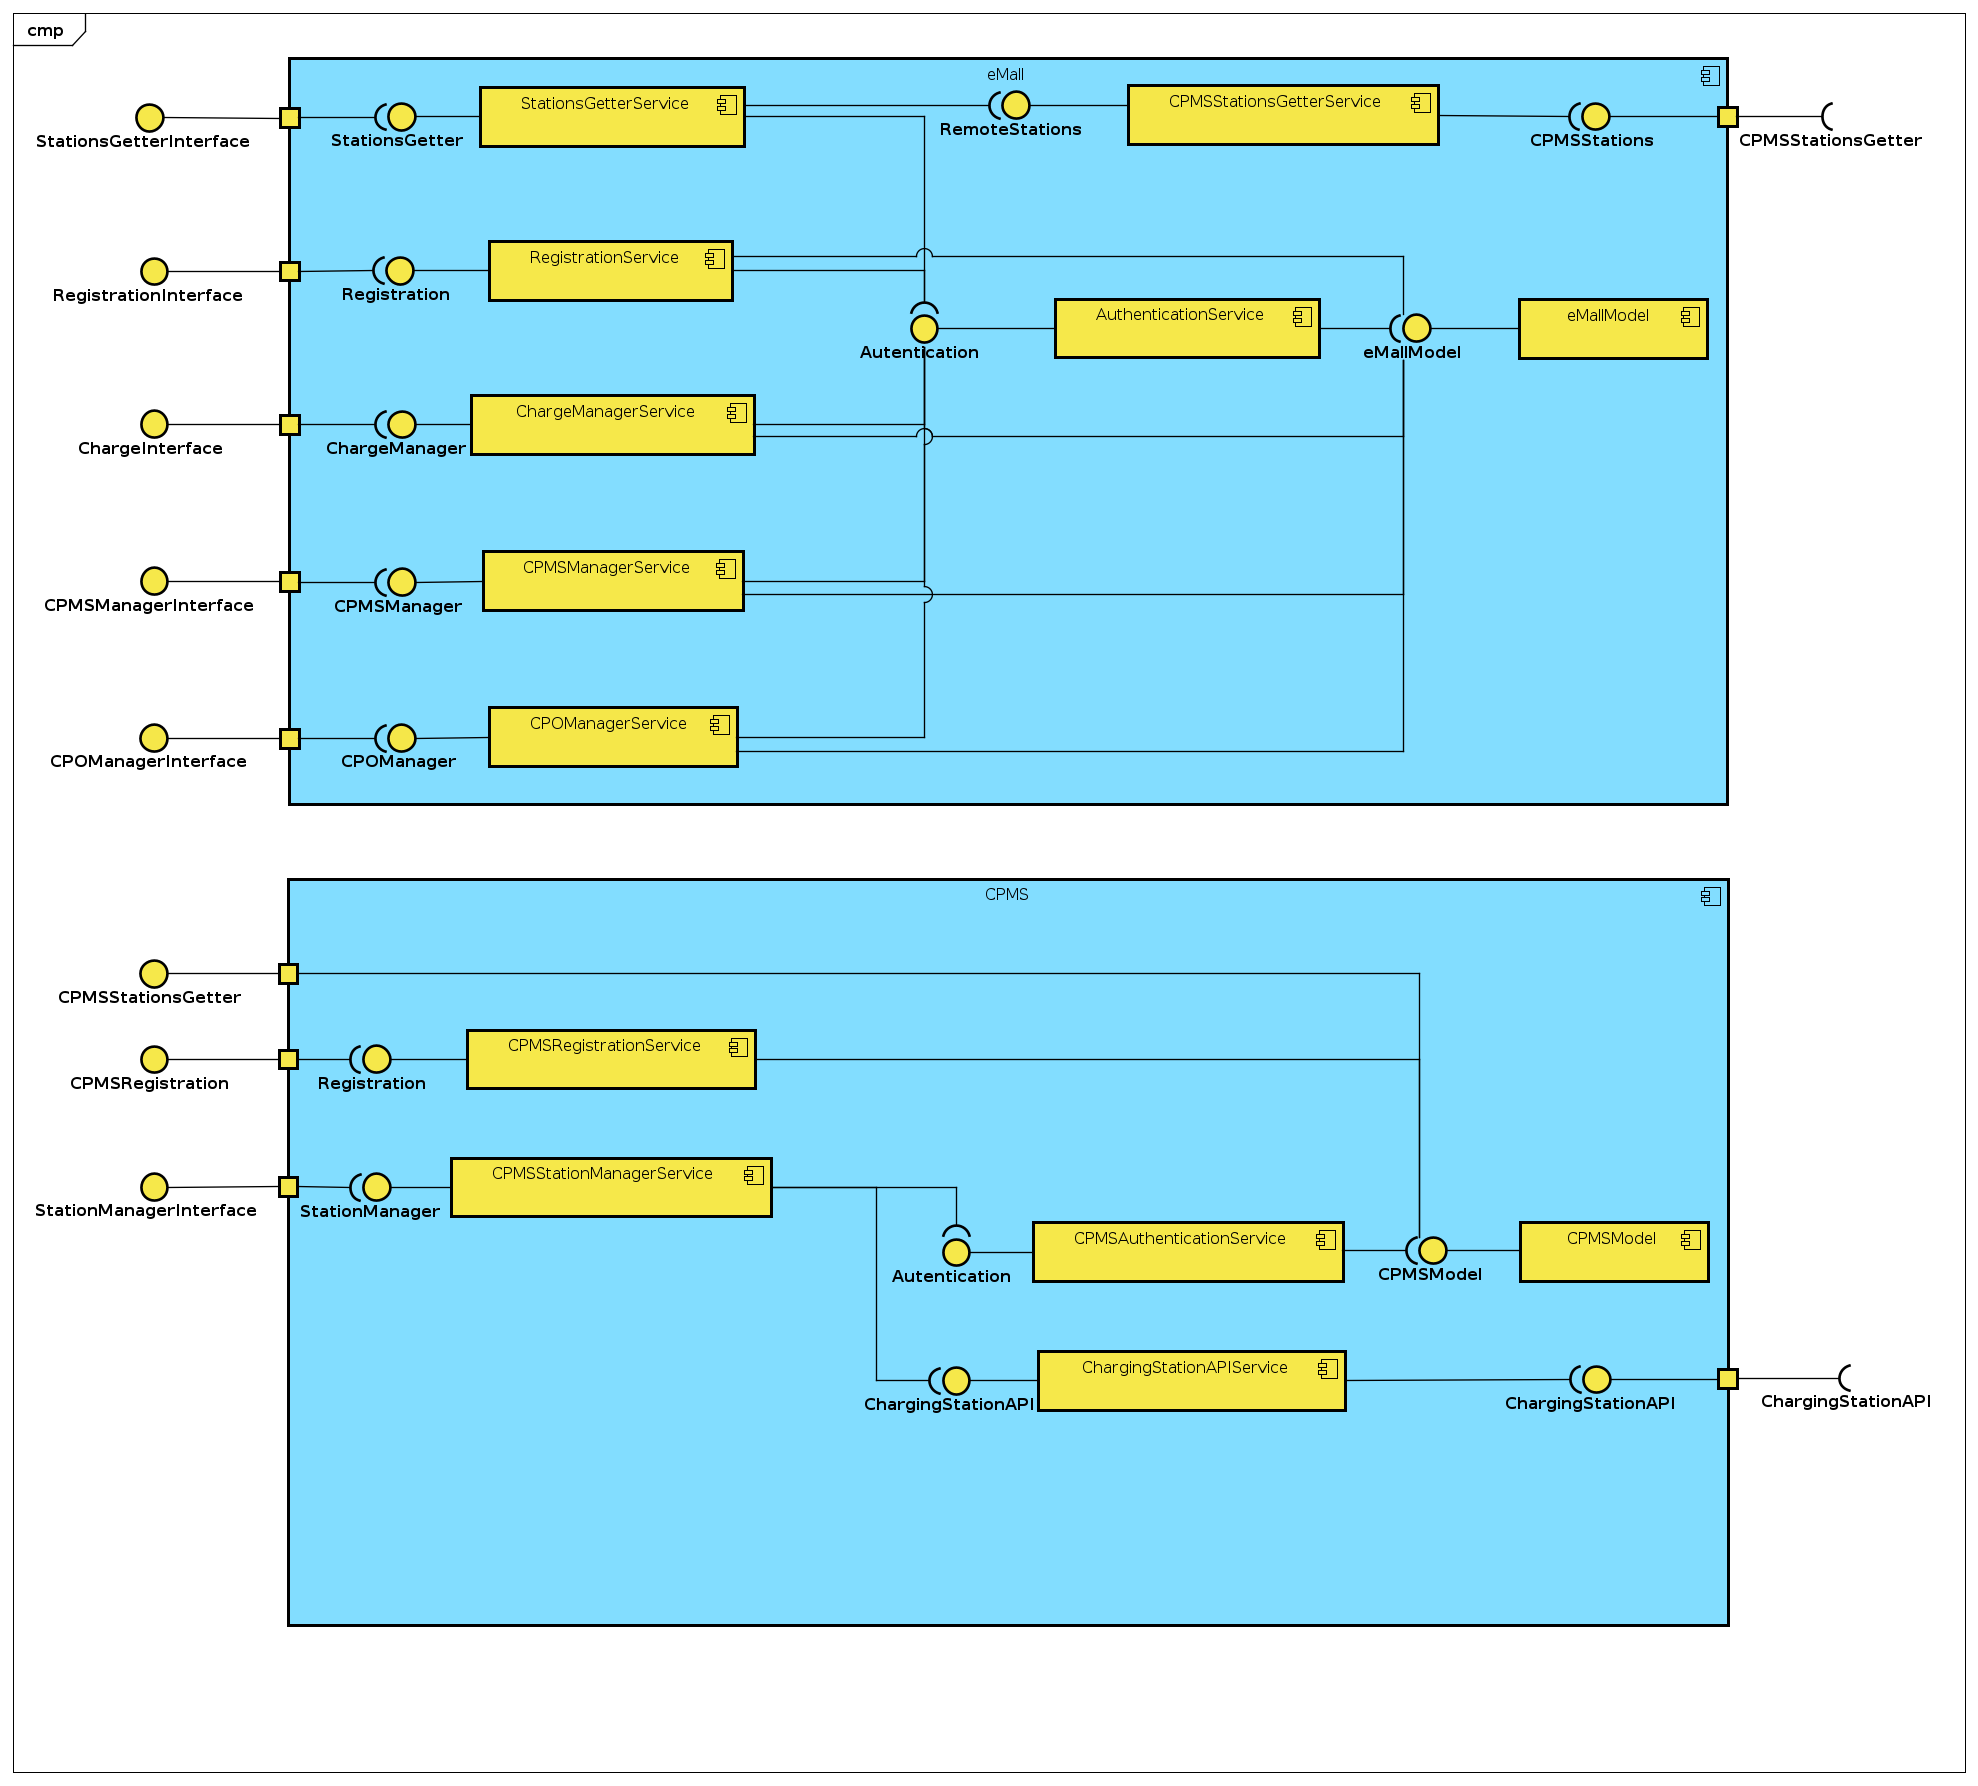
\includegraphics[keepaspectratio, width=16cm]{Component/Component.png}
        \caption{eMall component diagram}
        \label{fig:eMSP-component}
    \end{center}
\end{figure}
\clearpage
The two systems implement different interfaces and represent the \textit{Controller} and \textit{Model} parts of the \ac{MVC} pattern.
\makeatletter
\let\orgdescriptionlabel\descriptionlabel
\renewcommand*{\descriptionlabel}[1]{%
  \let\orglabel\label
  \let\label\@gobble
  \phantomsection
  \edef\@currentlabel{#1\unskip}%
  %\edef\@currentlabelname{#1}%
  \let\label\orglabel
  \orgdescriptionlabel{#1}%
}
\makeatother

\paragraph{\textbf{\ac{eMall}}}
The main components for the \ac{eMall} system are:
\begin{description}
    \item [\label{StationsComponent}StationsComponent] It is the component responsible for handling all the stations research requests (like \textit{getNearestStations}, \textit{getCheapestStation}, \textit{getTopKStationsNearby});
    \item [\label{RegistrationComponent}RegistrationComponent] It is the component responsible for handling the registration details along with the parameters checking during the registration phase;
    \item [\label{Timer}Timer] It is the component responsible of handling the registration verification timeout;
    \item [\label{ChargeManagerComponent}ChargeManagerComponent] It is the component responsible for handling all the charge booking/payment/cancellation processes. \\ It interfaces with the payment \ac{API} and with the charging station \ac{API};
    \item [\label{CPMSManagerComponent}CPMSManagerComponent] It is the component responsible for handling the \ac{CPMS} operations from the \acp{CPO} users;
    \item [\label{CPOManagerComponent}CPOManagerComponent] It is the component responsible for handling the \acp{CPO} requests (like \textit{SetRevenuePercentage} and \textit{setSpecialOffer});
    \item [\label{CPMSAPI}CPMS API] It is the component responsible for interfacing the \ac{eMall} with the CPMS interfaces;
    \item [\label{AuthenticationComponent}AuthenticationComponent] It is the component responsible for authorizing every operation over the model component. At this level it is implemented part of the controller (of the \ac{MVC} pattern) to check that operation is legit for the account type;
    \item [\label{MailAPI}Mail API] It is the component responsible for sending the feedback emails to the user every time an important operation is done;
    \item [\label{PaymentAPI}Payment API] It is a component that interfaces the \ac{eMall} system with the external payment \acp{API};
    \item [\label{eMallModel}eMall Model] It is the core component. It stores all the \ac{eMall} data and interfaces them with the other system components.
\end{description}
There are some apparently similar components with some slight differences:
\begin{itemize}
    \item The \ac{CPO} manager component is conceptually different from the \ac{CPMS} manager component because the CPMS manager Component alters the stations collection of the model according to the interface with the inserted \ac{CPMS};
\end{itemize}
\paragraph{\textbf{\ac{CPMS}}}
The main components for the \ac{CPMS} system are:
\begin{description}
    \item [\label{CPMSRegistrationComponent}CPMSRegistrationComponent] It is the component responsible for handling the registration details of new \ac{CPO} maintainers;
    \item [\label{CPMSStationManagerComponent}CPMSStationManagerComponent] It is the component responsible for handling all the station managing actions from a \ac{CPO} maintainer (\textit{setStationStrategy}, \textit{setStationSource}..);
    \item [\label{CPMSChargeManagerComponent}CPMSChargeManagerComponent] It is the component responsible for handling all the actions which involve book/enable/cancel a charge. The \ac{eMall} is the only component that utilizes this interface;
    \item [\label{CPMSAuthenticationComponent}CPMSAuthenticationComponent] It is the component responsible for authorizing every operation over the model component. At this level it is implemented part of the controller (of the \ac{MVC} pattern) to check that operation is legit;
    \item [\label{CPMSChargingStationAPI}CPMSChargingStation API] It is the component that interfaces the \ac{CPMS} system with the external Charging Stations;
    \item [\label{CPMSModel}CPMSModel] It is the core component. It stores all the \ac{CPMS} data and interfaces them with the other system components.
\end{description}
In the component diagrams, there are components (\textit{Payment\ac{API}}, \textit{\ac{CPMS}\ac{API}}, \textit{Mail\ac{API}}, \\\textit{\ac{CPMS}ChargingStationAPI}) that could be bypassed, letting the main components interface the external \acp{API}. These components are integrated because they offer the possibility to contain the external interface standards in one single component. This creates the possibility for developers to create an internal interfacing standard different from the external ones.

\subsection{Deployment view}
The general idea of the deployment view is to show all the principal architectural components with the distribution of the artifacts (applications, firewall rule tables, data\ldots).

\subsubsection{\ac{eMSP}}
\begin{figure}[!h]
    \begin{center}
        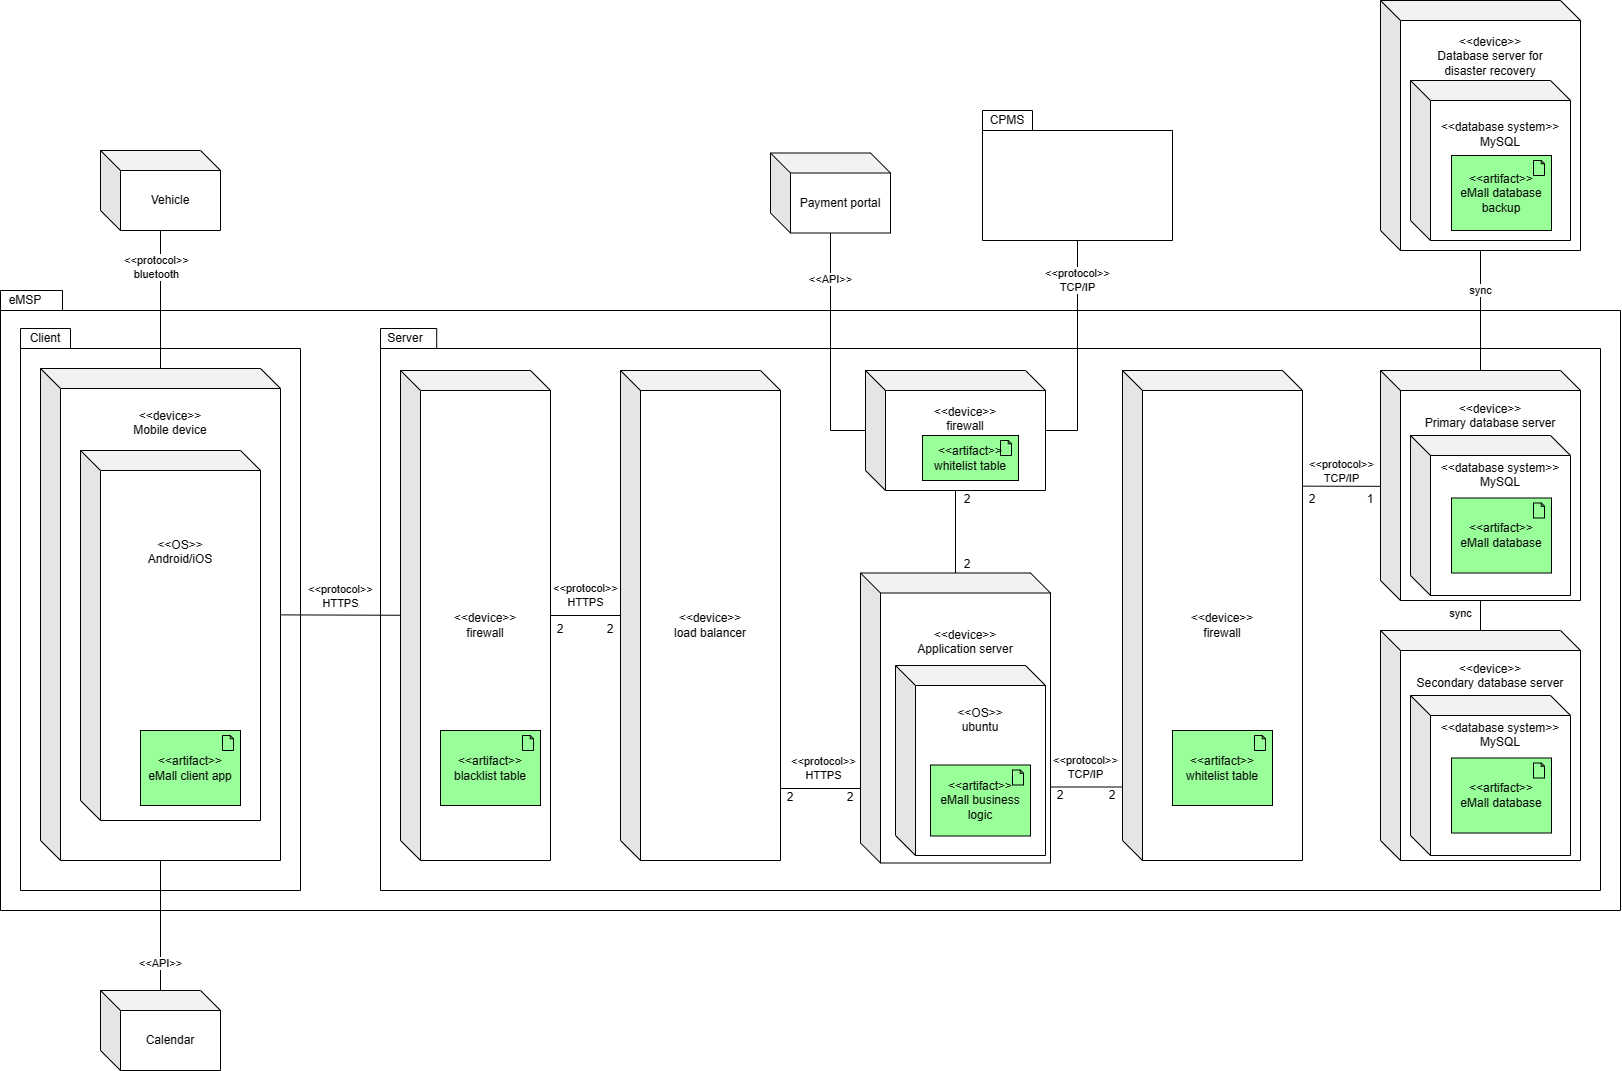
\includegraphics[keepaspectratio, width=0.9\textwidth]{Graphics/DD-eMSP-deployment.drawio.png}
        \caption{eMall deployment view diagram}
        \label{fig:eMSP-deployment}
    \end{center}
\end{figure}

The system has been designed in order to avoid \acp{SPOF}, in order to be used by an high availability service, and to support security policies. So the components of the system are:
\begin{itemize}
    \item Mobile device: It is the device used by users or \acp{CPO} to interact with the \ac{eMall} system. It is provided with internet connection, bluetooth peripheral and the \ac{eMall} client application installed. This application must be available for both Android and iOS mobile operative systems in order to be available by the most part of the people.
          Uses \ac{HTTPS} to communicate with the server or the calendar in order to exploit all the security layers implemented by it, following, in this way, also the \ac{GDPR} law. Uses bluetooth (or whatever protocol used by vehicles to create a PAN) in order to retrieve vehicle infos.
    \item Application server: server that receives all the requests from the clients and hosts the business logic. There are two redundant application servers in order to increase reliability and availability while also avoiding down-times while maintaining the \ac{eMall} service.
    \item Load balancer: balances the load of the requests on the different application servers and handles the case if one application server is down. This system provides failover as described in \cite{ref:redundant-load-balancers}.
    \item Firewall: Each firewall in the server is used to isolate different zones. A first firewall interfaces the external world to the load balancer in order to filter dangerous requests.
          Blacklist rule table is implemented for the impossibility to implement an allowlist. For the firewall that interfaces the application server to the database an allowlist rule table is implemented because the only traffic permitted to the database is the one coming from the application servers. This system provides failover as described in \cite{ref:redundant-firewalls}.
    \item Database system: A redundant database system is implemented where the secondary database should always be synced with the primary in order to be ready for substituting the primary one in case of failure as described in \cite{ref:redundant-databases}. Also a disaster recovery database is necessary since data is of primary importance in this application. MySQL DBMS has been chosen because it is one of the most used relational DBMS \cite{ref:most-popular-RDBMS}.
\end{itemize}
\todo[inline]{Protocol used: (application server - CPMS) and (user device - server)}
\subsubsection{\ac{CPMS}}
\begin{figure}[!h]
    \begin{center}
        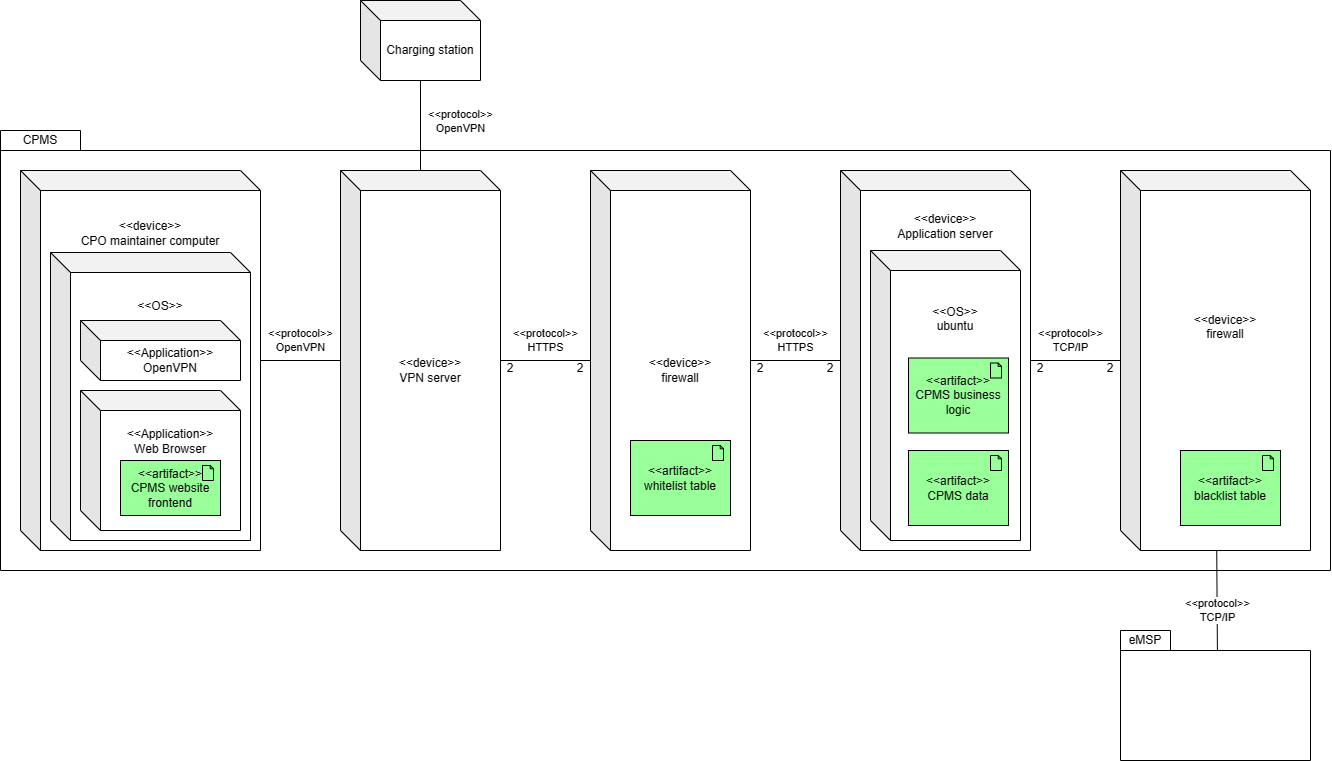
\includegraphics[keepaspectratio, width=0.9\textwidth]{Graphics/DD-CPMS-deployment.drawio.png}
        \caption{CPMS deployment view diagram}
        \label{fig:CPMS-deployment}
    \end{center}
\end{figure}

For the \ac{CPMS} the concept is to keep all the communication as in a private network, implementing a \ac{VPN} for the remote nodes (i.e. the \ac{CPO} maintainer personal computer and the charging stations) so that only people in that \ac{VPN} have the ability to perform maintainer's actions. The only point where remote connections happen is from \acp{eMSP}. Another important factor is the redundancy of the systems, in order to avoid \acp{SPOF}.
\begin{itemize}
    \item \ac{CPO} maintainer computer: This device is connected through a \ac{VPN} to a \ac{VPN} server. It runs the management software for the \ac{CPMS} the maintainer wants to administrate on top of an Ubuntu operative system, the most used linux distro according to \cite{ref:most-popular-linux-distro}.
          In our architecture this is the thin client, in fact the \ac{CPMS} management software just handles the view of the information retrieved and sends commands to the application server. All the business logic will be contained in the application server.
    \item \ac{VPN} server: It permits the \ac{CPO} maintainer computers, the charging stations and the application server to share the same network in order to simplify the communication among the components.
          The OpenVPN protocol \cite{ref:openvpn-site} has been chosen because it is an open source project and is very widely used in many different applications. This system provides failover as described in \cite{ref:redundant-VPN-servers}.
    \item Application server: This is the component that handles all the commands issued to the system and redirects them to the charging stations if needed. It is surrounded by firewalls so that we can enforce security policies, such as blocking particular public IPs or allow only some internal IPs corresponding to the charging stations or the \ac{CPO} maintainer computers. This system is redundant in order to assure the continuity of availability during maintenance.
    \item Firewalls:
\end{itemize}
\todo[inline]{Added <<API>>}
\todo[inline]{Protocol used: (eMSP - application server)}
\clearpage

\subsection{Runtime view}
\todo[inline]{Implementare CPO rimuove CPMS da eMall anche nel RASD.}
\todo[inline]{Controllare che ci sia l'assunzione nel RASD per cui alla prima accensione il primo CPOmaintainer viene impostato.}
\begin{figure}[!h]
    \begin{center}
        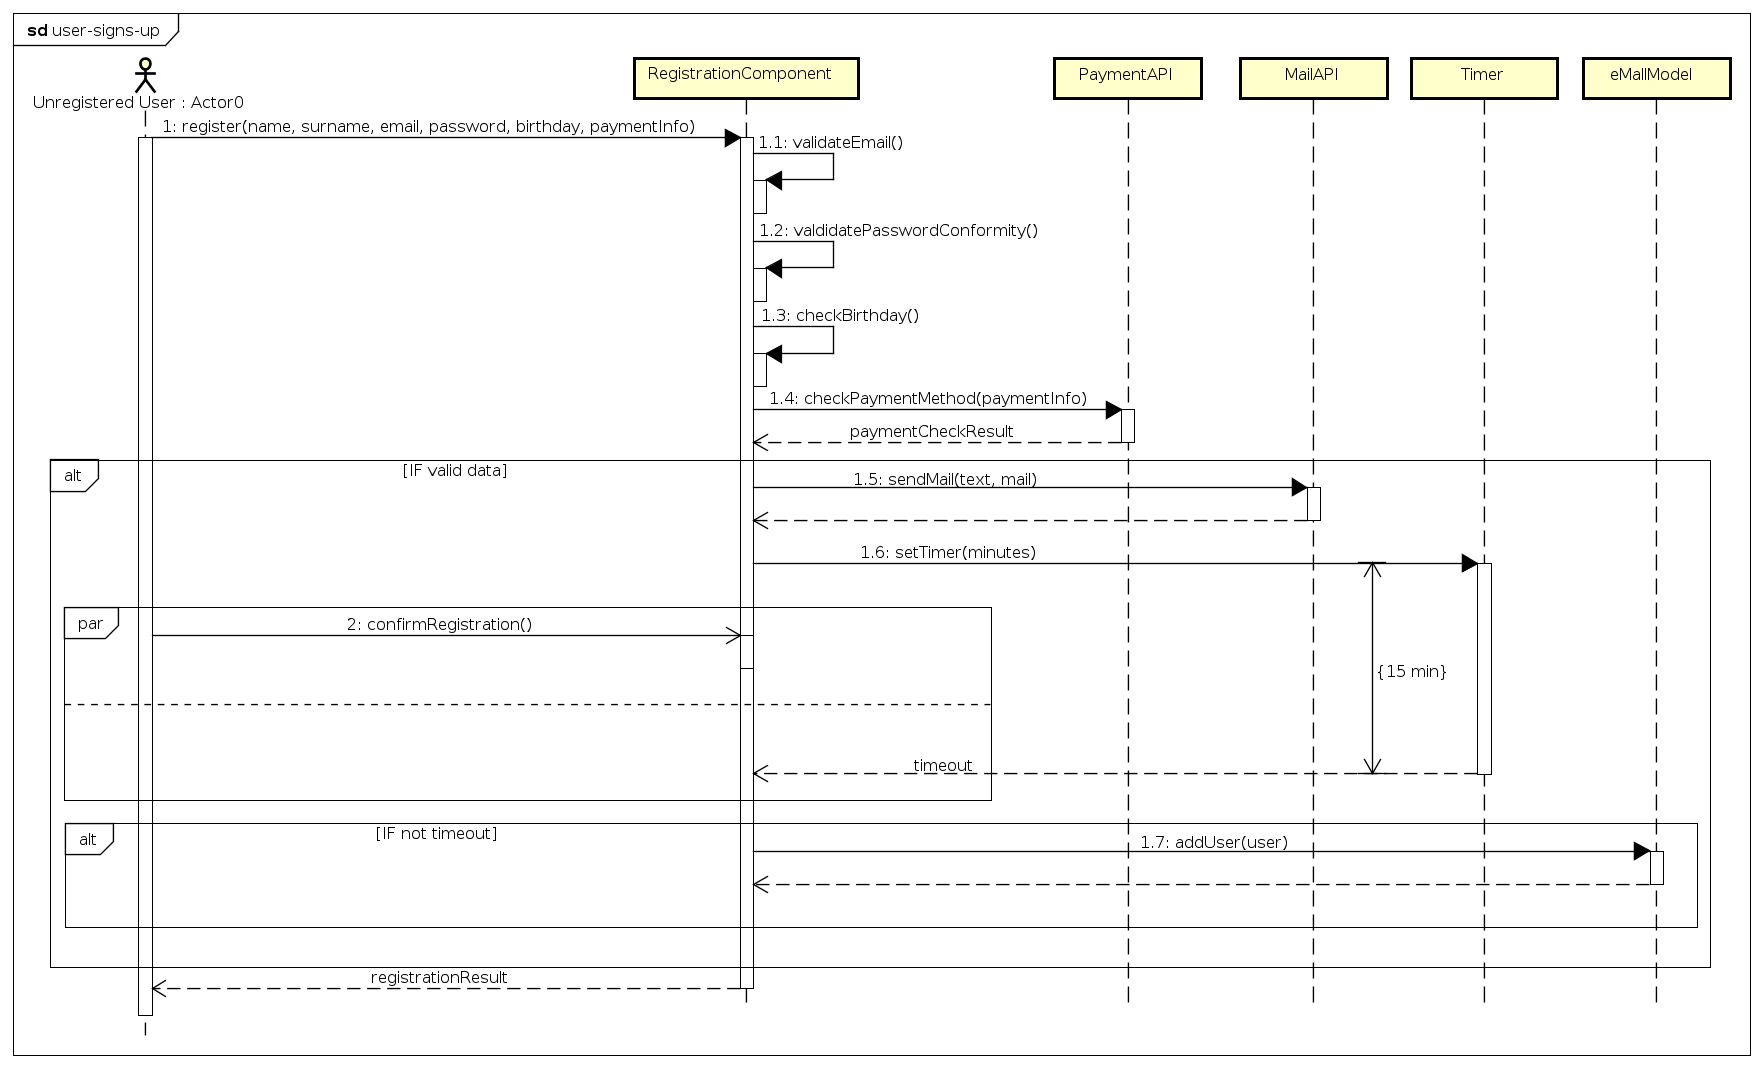
\includegraphics[keepaspectratio, width=16cm]{Sequence/user-signs-up.png}
        \caption{User signs up}
        \label{fig:user-signs-up}
    \end{center}
\end{figure}
\begin{figure}[!h]
    \begin{center}
        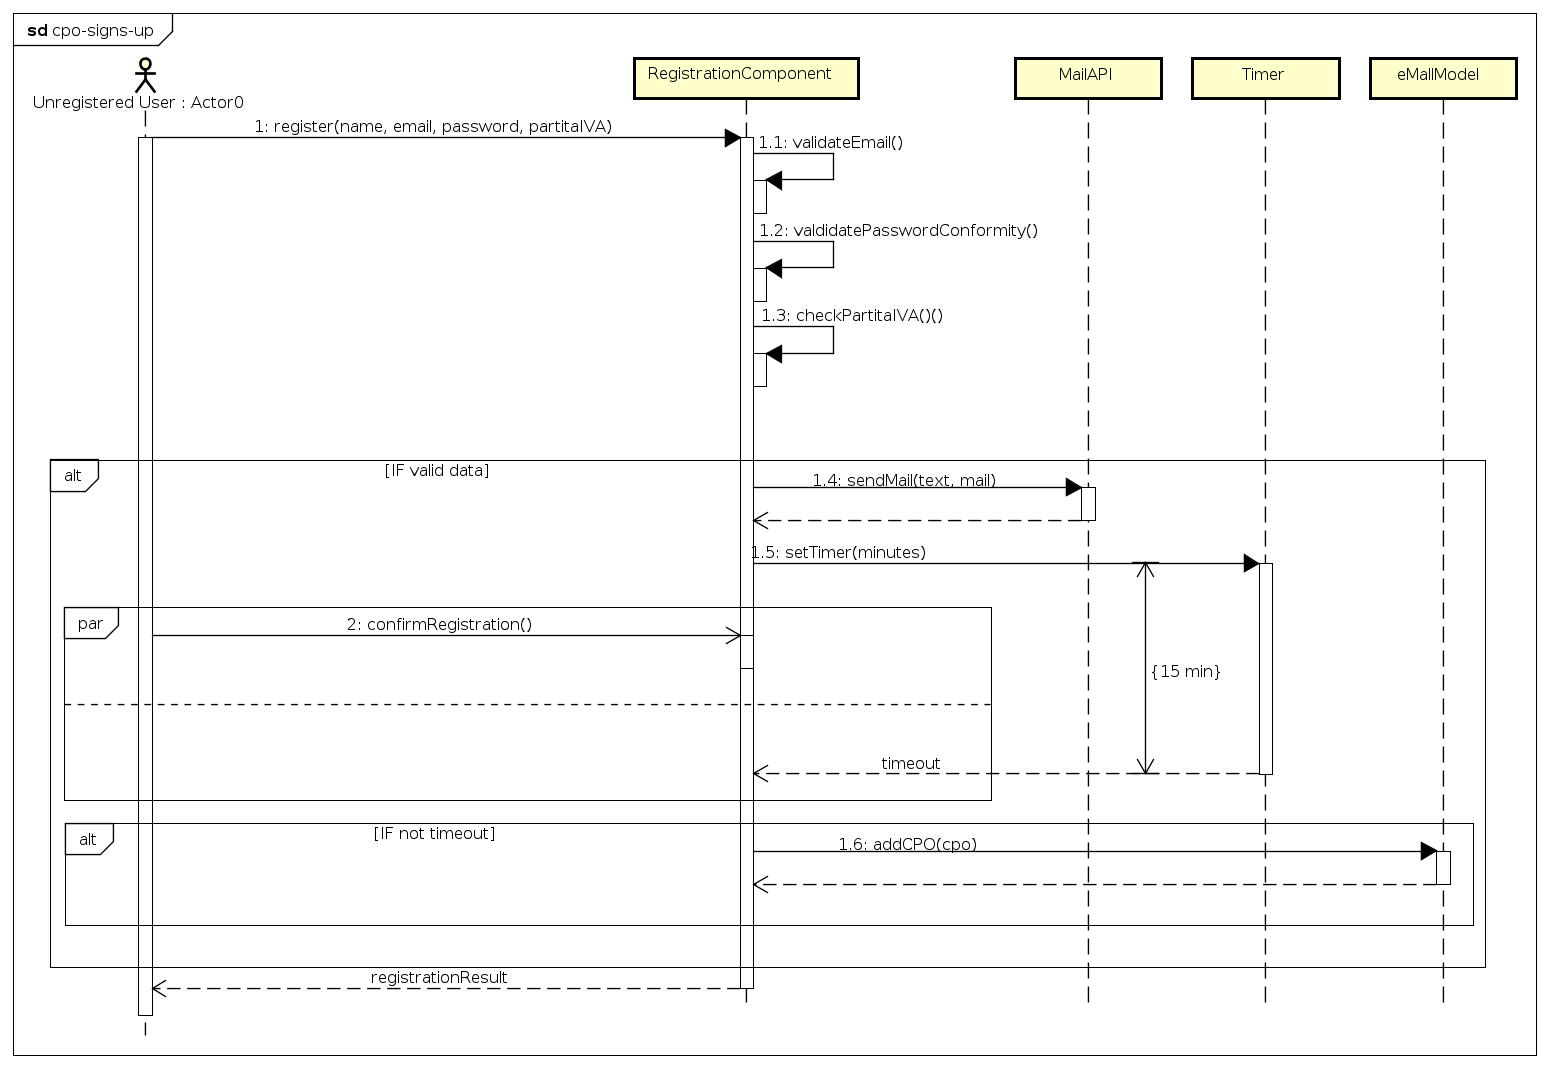
\includegraphics[keepaspectratio, width=16cm]{Sequence/cpo-signs-up.png}
        \caption{\ac{CPO} signs up}
        \label{fig:cpo-signs-up}
    \end{center}
\end{figure}
\begin{figure}[!h]
    \begin{center}
        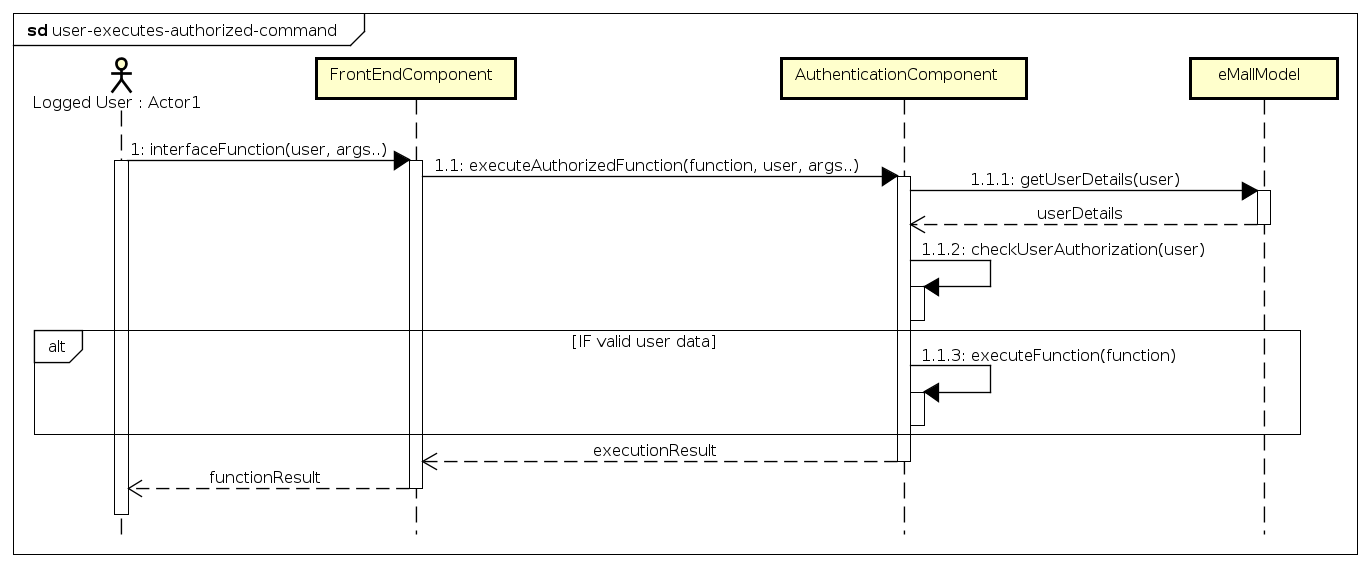
\includegraphics[keepaspectratio, width=16cm]{Sequence/user-executes-authorized-command.png}
        \caption{User executes authorized command}
        \label{fig:user-executes-authorized-command}
    \end{center}
\end{figure}
\begin{figure}[!h]
    \begin{center}
        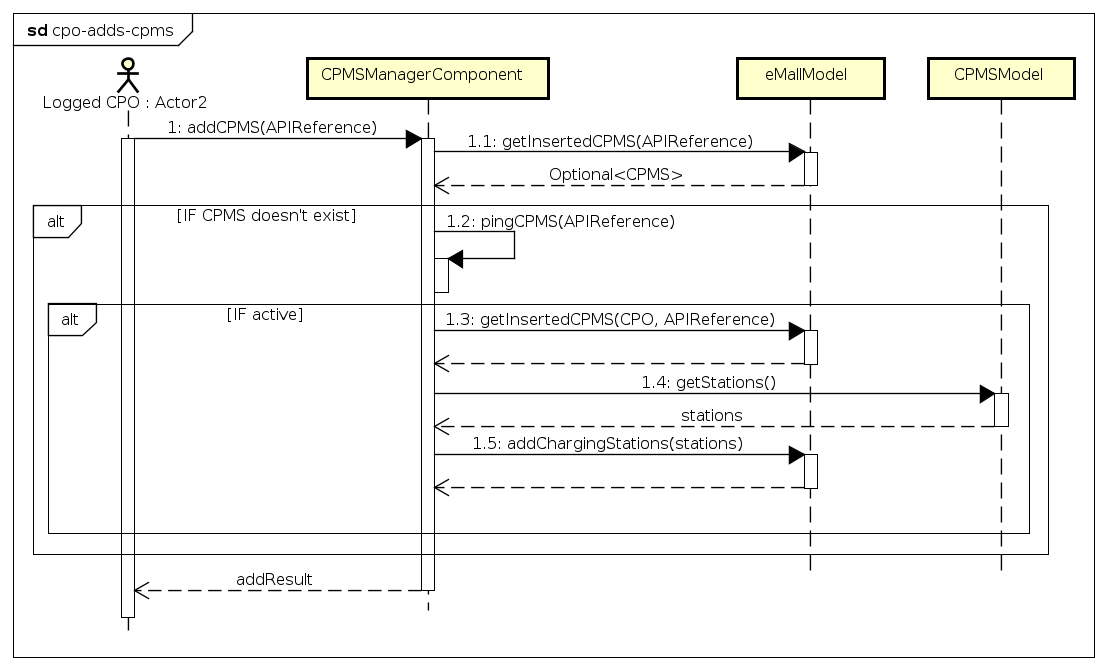
\includegraphics[keepaspectratio, width=16cm]{Sequence/cpo-adds-cpms.png}
        \caption{\ac{CPO} adds \ac{CPMS} into \ac{eMall}}
        \label{fig:cpo-adds-cpms}
    \end{center}
\end{figure}
\begin{figure}[!h]
    \begin{center}
        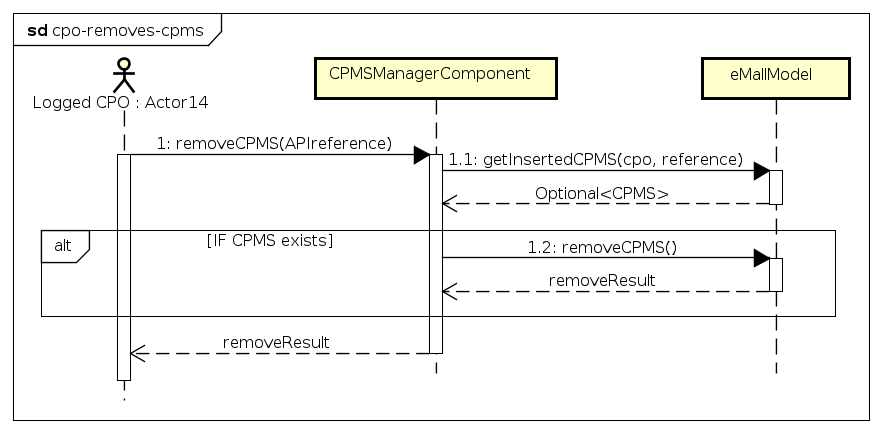
\includegraphics[keepaspectratio, width=16cm]{Sequence/cpo-removes-cpms.png}
        \caption{\ac{CPO} removes \ac{CPMS} from \ac{eMall}}
        \label{fig:cpo-removes-cpms}
    \end{center}
\end{figure}
\begin{figure}[!h]
    \begin{center}
        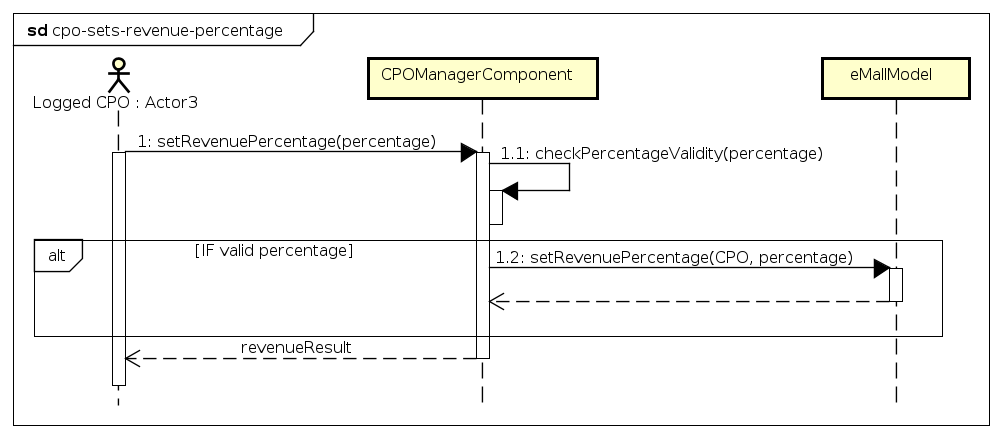
\includegraphics[keepaspectratio, width=16cm]{Sequence/cpo-sets-revenue-percentage.png}
        \caption{\ac{CPO} sets the revenue percentage}
        \label{fig:cpo-sets-revenue-percentage}
    \end{center}
\end{figure}
\begin{figure}[!h]
    \begin{center}
        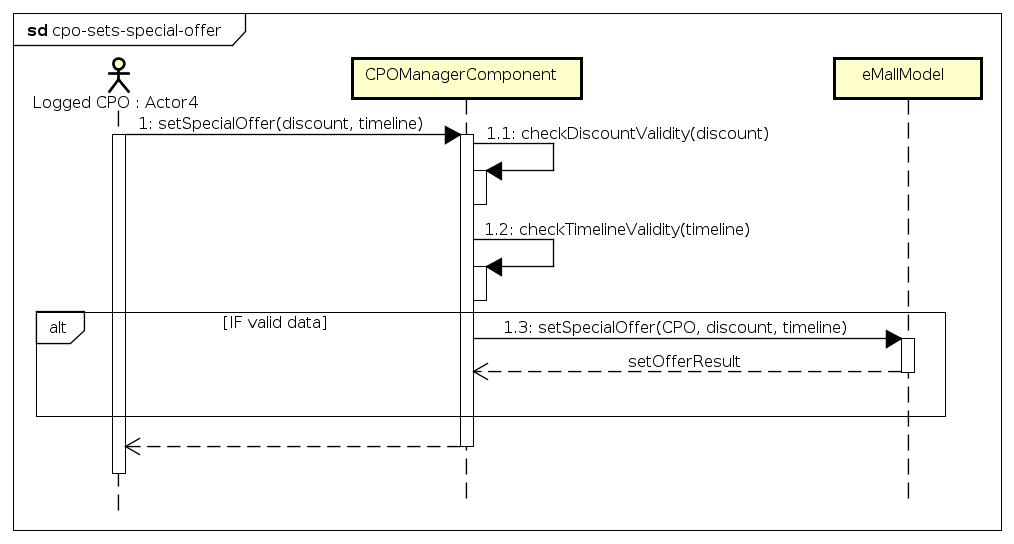
\includegraphics[keepaspectratio, width=16cm]{Sequence/cpo-sets-special-offer.png}
        \caption{\ac{CPO} sets a special offer}
        \label{fig:cpo-sets-speciale-offer}
    \end{center}
\end{figure}
\begin{figure}[!h]
    \begin{center}
        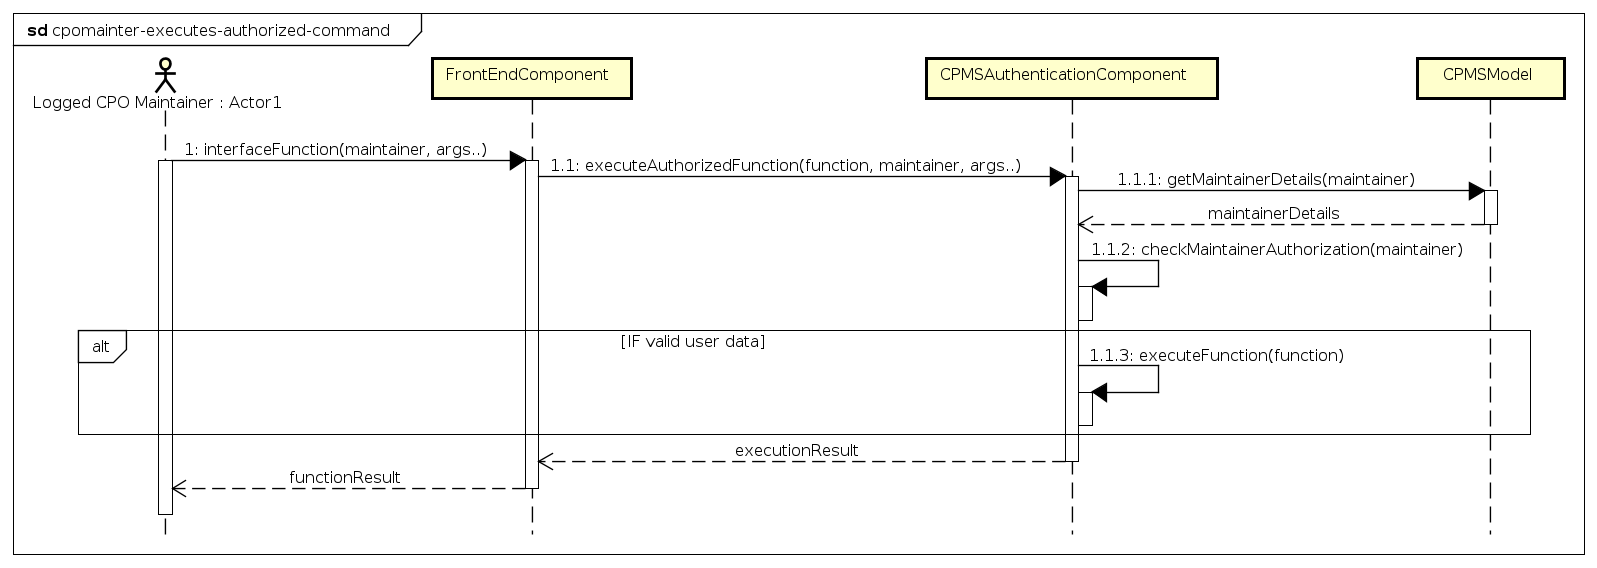
\includegraphics[keepaspectratio, width=16cm]{Sequence/cpomaintainer-executes-authorized-command.png}
        \caption{\ac{CPO}maintainer executes authorized command}
        \label{fig:cpomaintainer-executes-authorized-command}
    \end{center}
\end{figure}
\begin{figure}[!h]
    \begin{center}
        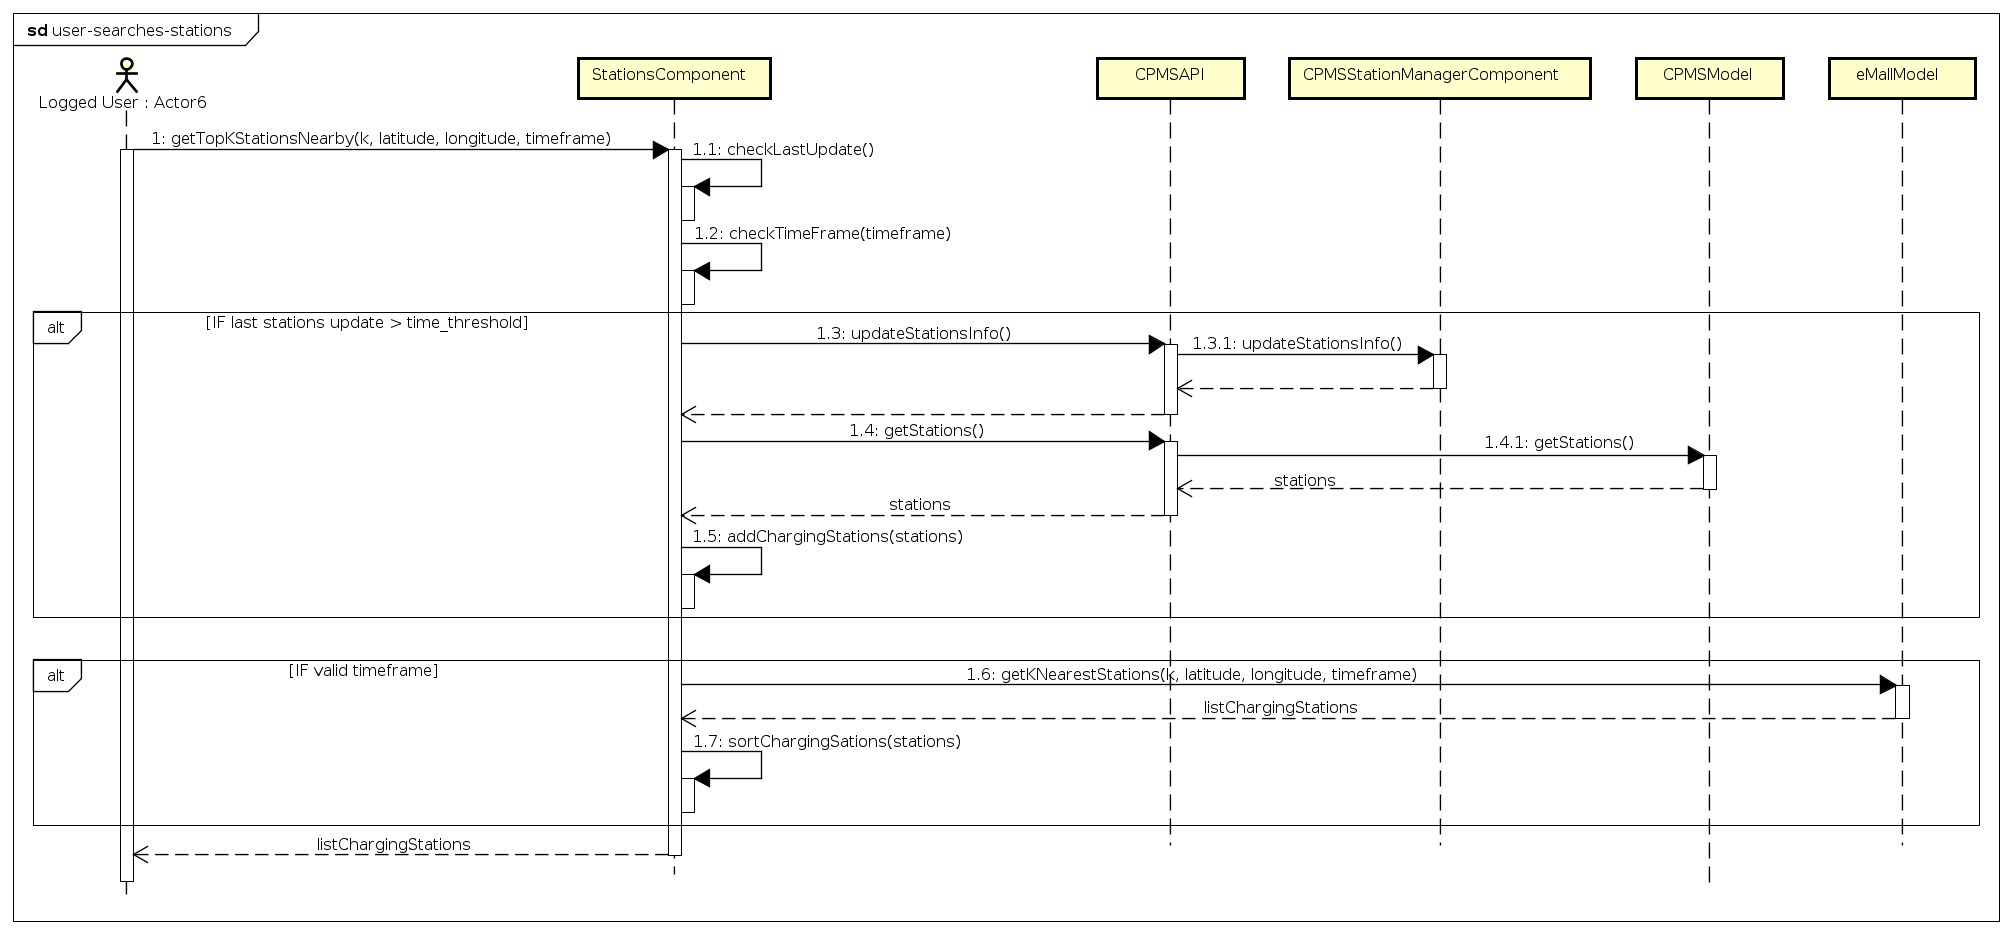
\includegraphics[keepaspectratio, width=16cm]{Sequence/user-searches-stations.png}
        \caption{Get the nearby charging stations}
        \label{fig:user-searches-stations}
    \end{center}
\end{figure}
\begin{figure}[!h]
    \begin{center}
        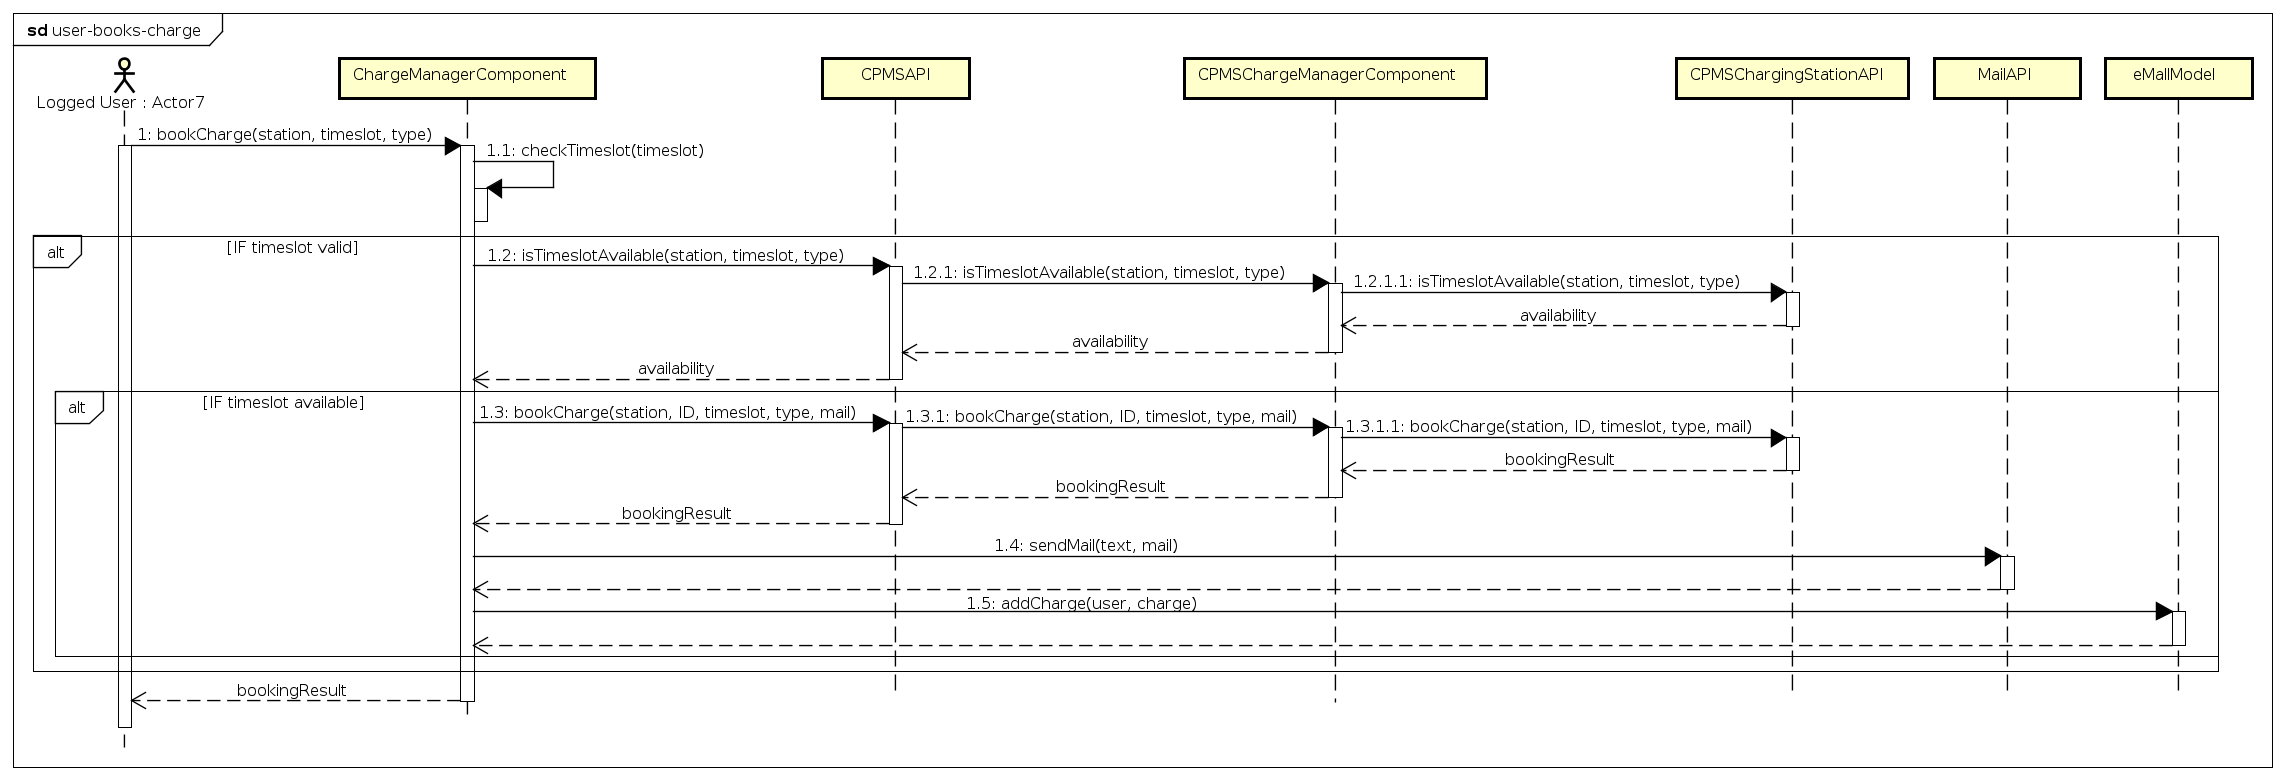
\includegraphics[keepaspectratio, width=16cm]{Sequence/user-books-charge.png}
        \caption{Book a charge sequence}
        \label{fig:user-books-charge}
    \end{center}
\end{figure}
\begin{figure}[!h]
    \begin{center}
        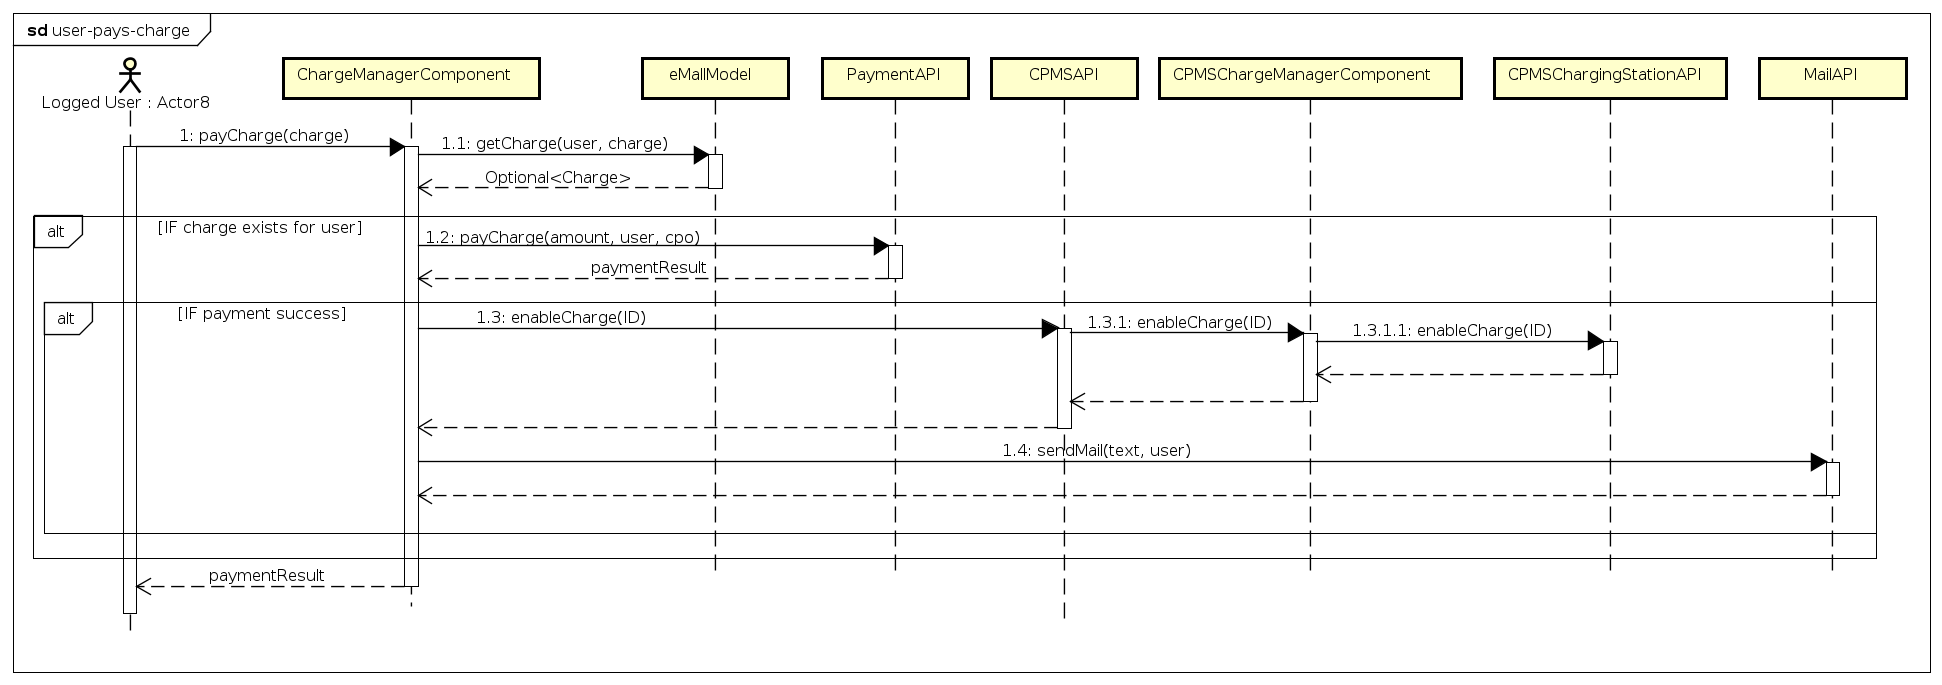
\includegraphics[keepaspectratio, width=16cm]{Sequence/user-pays-charge.png}
        \caption{Pay a charge sequence}
        \label{fig:user-pays-charge}
    \end{center}
\end{figure}
\begin{figure}[!h]
    \begin{center}
        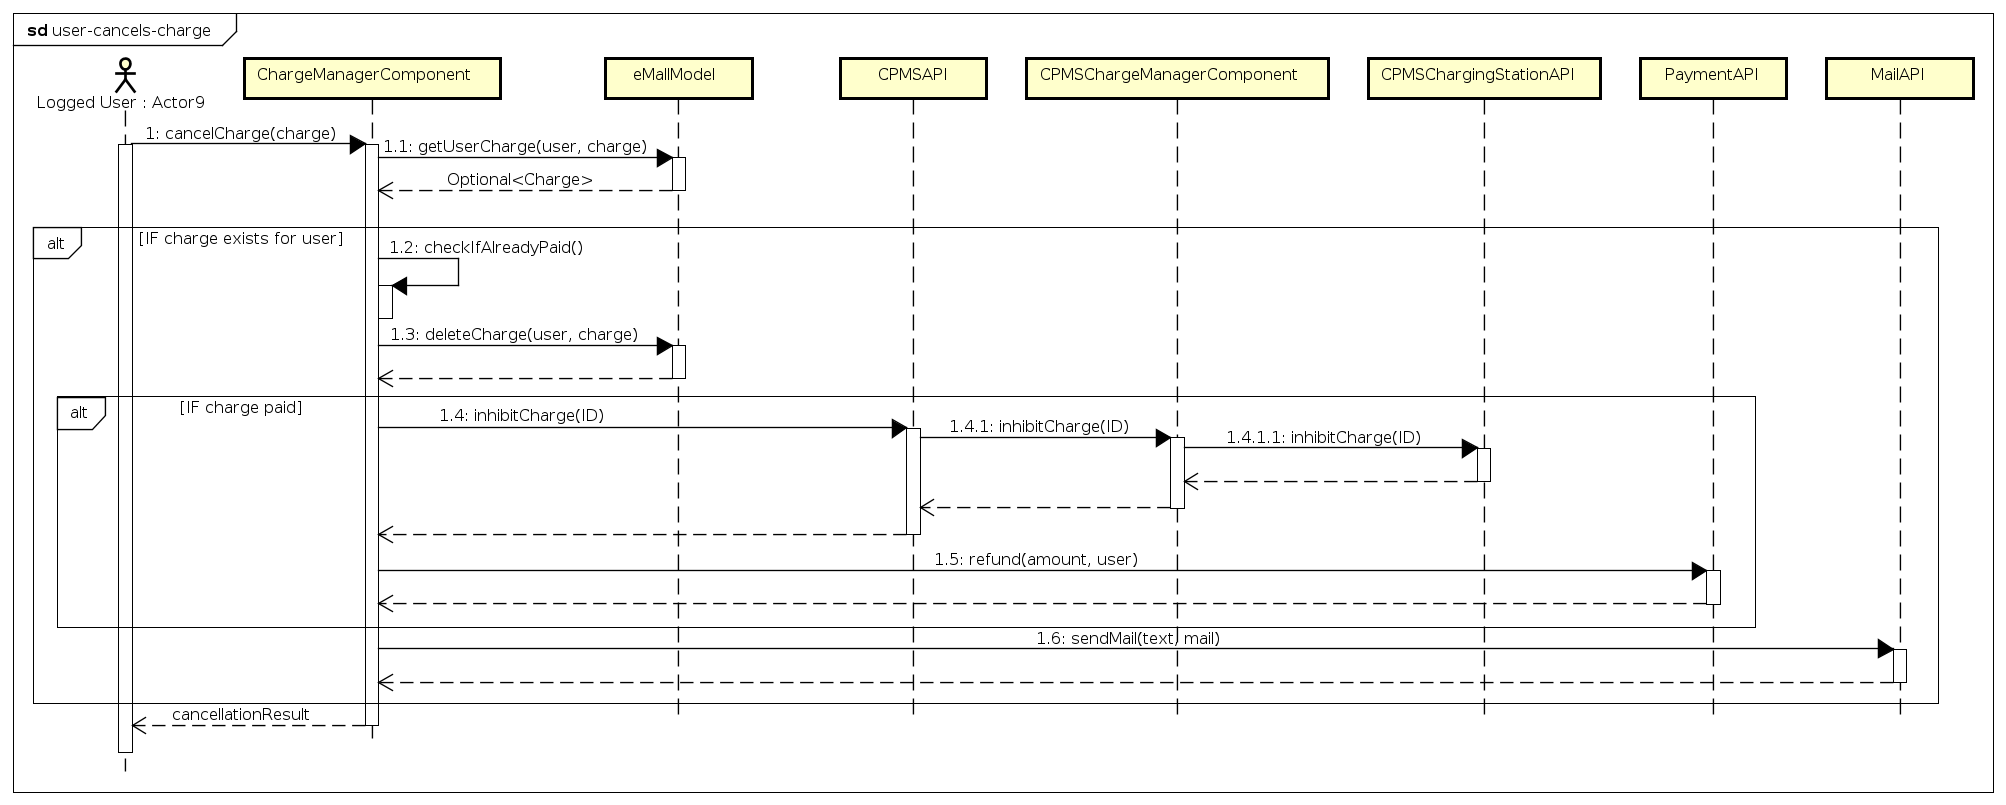
\includegraphics[keepaspectratio, width=16cm]{Sequence/user-cancels-charge.png}
        \caption{Cancel a charge sequence}
        \label{fig:user-cancels-charge}
    \end{center}
\end{figure}
\begin{figure}[!h]
    \begin{center}
        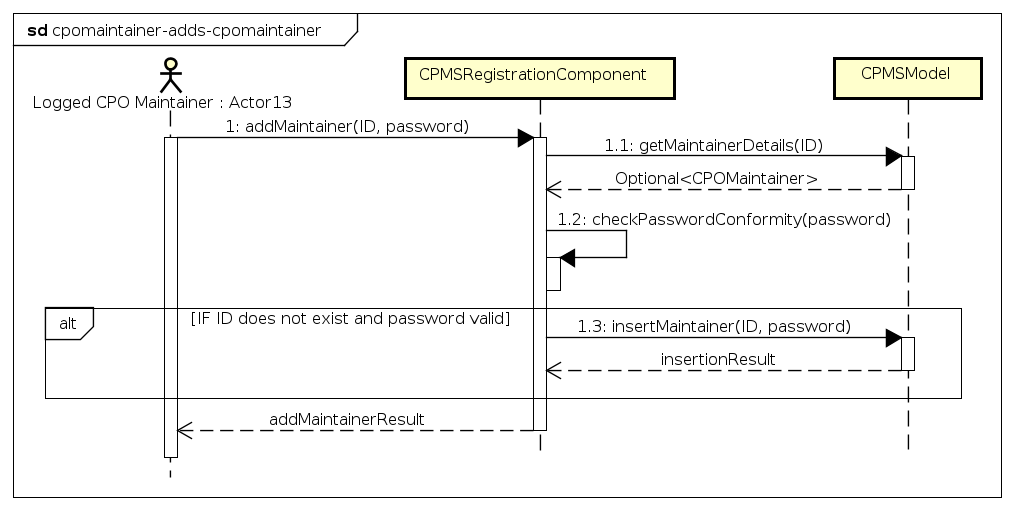
\includegraphics[keepaspectratio, width=16cm]{Sequence/cpomaintainer-adds-cpomaintainer.png}
        \caption{\ac{CPO}maintainer adds \ac{CPO}maintainer to \ac{CPMS}}
        \label{fig:cpomaintainer-adds-cpomaintainer}
    \end{center}
\end{figure}
\begin{figure}[!h]
    \begin{center}
        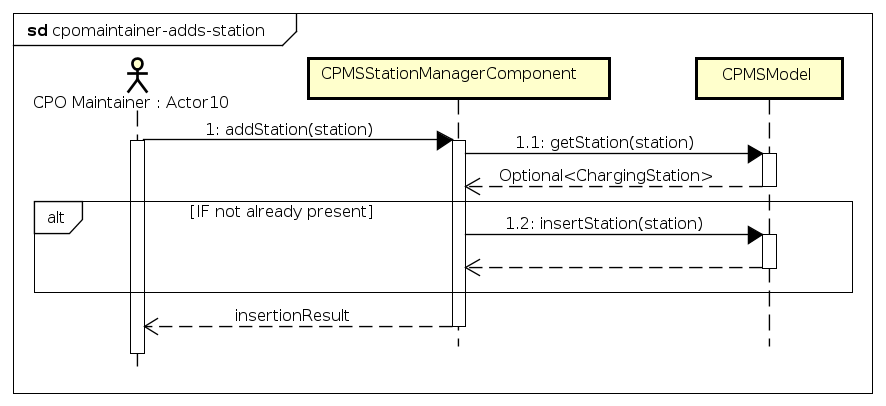
\includegraphics[keepaspectratio, width=16cm]{Sequence/cpomaintainer-adds-stations.png}
        \caption{\ac{CPO}maintainer adds stations to \ac{CPMS}}
        \label{fig:cpomaintainer-adds-stations}
    \end{center}
\end{figure}
\begin{figure}[!h]
    \begin{center}
        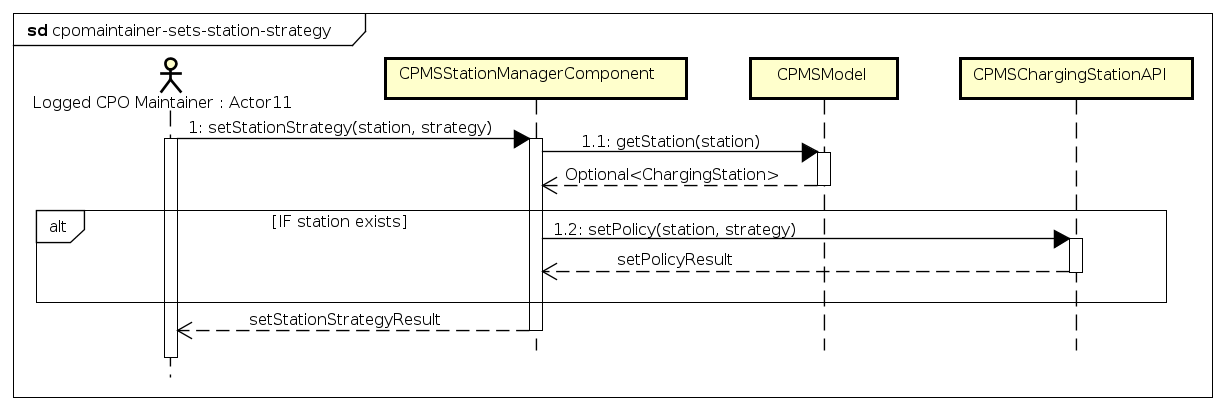
\includegraphics[keepaspectratio, width=16cm]{Sequence/cpomaintainer-sets-station-strategy.png}
        \caption{\ac{CPO}maintainer sets station strategy in \ac{CPMS}}
        \label{fig:cpomaintainer-sets-station-strategy}
    \end{center}
\end{figure}
\begin{figure}[!h]
    \begin{center}
        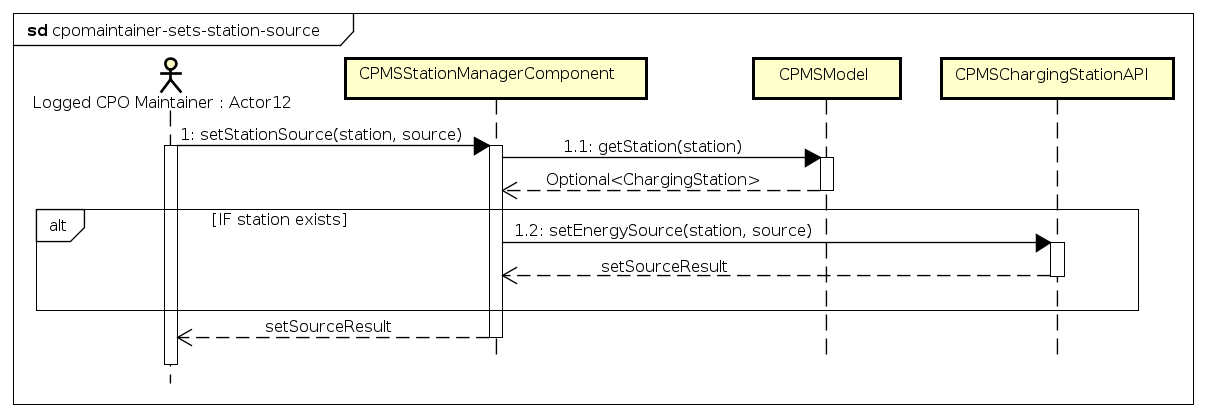
\includegraphics[keepaspectratio, width=16cm]{Sequence/cpomaintainer-sets-station-source.png}
        \caption{\ac{CPO}maintainer sets station source in \ac{CPMS}}
        \label{fig:cpomaintainer-sets-station-source}
    \end{center}
\end{figure}
\clearpage
There are some particular design decisions that need to be clarified:
\begin{itemize}
    \item \textbf{Login sequences:} In \autoref{fig:user-executes-authorized-command} and \autoref{fig:cpomaintainer-executes-authorized-command} it is illustrated the way the system authorizes \acp{CPO} and users. The idea is to filter authorized commands using functions (like \cite{ref:command-pattern}). The component that filters the requests is the AuthorizationComponent (present in both \ac{eMall} and \ac{CPMS} systems).\\
          When the client utilizes the interface, automatically it has to send also his credentials; these are then verified by the AuthorizationComponent and, if correct it executes the corresponding API function. This pattern allows the system to decentralize the authorization verification from the API code and allows every function that needs this data to have access to the client's account information;
    \item \textbf{Asynchronous messages:} During the inter-system communications (like \ac{eMall} -> \ac{CPMS} or \ac{CPMS} -> ChargingStation) it would be useful to implement asynchronous communications to avoid blocking situations. However in the sequence diagrams there aren't any because a better solution (compromise between having a completely asynchronous communication and having feedback from the interface) is to implement a timeout timer to avoid a complete block. This information is not shown in the sequence diagrams due to its verbosity of notation.

\end{itemize}
\subsection{Component interfaces}


\subsection{Selected architectural styles and patterns}
\begin{itemize}
    \item Bridge pattern \cite{ref:bridge-pattern}: It consists in decoupling completely two systems by having two interfaces. In \autoref{fig:bridge-pattern} there is a simplification of the architecture in order to highlight the usage of this pattern.
          Instead of having a great system with the composition of an \ac{eMSP} and a \ac{CPMS} we exploit their interfaces in order to implement in a decoupled way these two systems. So, the \ac{eMSP} implementation (i.e. \ac{eMall}) will interact with a \ac{CPMS} implementation through his interface.
\end{itemize}
\todo[inline]{migliorare qualità immagine}
\begin{figure}[!h]
    \begin{center}
        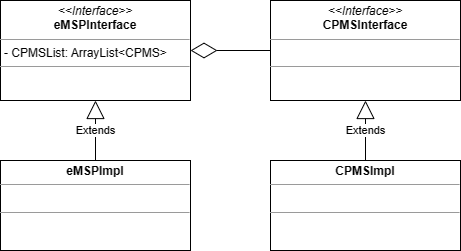
\includegraphics[keepaspectratio, width=16cm]{Graphics/DD-bridge-pattern.drawio.png}
        \caption{Bridge pattern representation in the system}
        \label{fig:bridge-pattern}
    \end{center}
\end{figure}

\subsubsection{\ac{eMSP} architectural styles and patterns}
\begin{itemize}
    \item \acl{MVC} pattern \cite{ref:MVC-pattern}: It consists in grouping the system in three clusters:
          \begin{itemize}
              \item the model, with all the persistent data of the system;
              \item the view, with the logic to present the model;
              \item the controller, with the business logic for elaborating requests from the view and manipulating the model.
          \end{itemize}
          In this context, the pattern makes easy to separate and decouple the model (distributed on the database), the view (distributed on the client application) and the controller.
          This last component is then divided into two classes:
          the first, distributed on the client, consists in the elaboration of the data retrieved from the calendar or the vehicle in order to send to the server very small requests;
          the second, distributed on the application server, takes care of handling the requests made by the client and interacting with the model.
    \item Three-tier architecture \cite{ref:multitier-pattern}: In order to increase modularity and manageability of the system, the division among presentation, application and data tiers is used. This also makes it possible to improve just one tier without having to touch the other two.
    \item \ac{DAO} pattern \cite{ref:dao-pattern}: This pattern permits to map directly the relational tables in the database to objects in the application. It permits to decouple more the application layer and the data layer.
\end{itemize}

\subsubsection{\ac{CPMS} architectural styles and patterns}
\begin{itemize}
    \item \acl{MVC} pattern \cite{ref:MVC-pattern}: In this case we use this pattern in order to decouple the view logic from the rest. Also, this simplifies the organization and implementation of the codebase. In addition, here too we can benefit from having a software layer that handles the access to the model and avoid that the presentation layer directly accesses the model.
    \item Two-tier architecture \cite{ref:multitier-pattern}: Since the \ac{CPMS} shouldn't handle the amount of traffic of an \ac{eMSP} system, the \ac{CPMS} is simpler and only distributed on 2 tiers: a thin-client with only the presentation layer which handles the view logic and an application server.
\end{itemize}


\subsection{Other design decisions}
\subsubsection{\ac{SPOF} avoidance}
In both the \ac{eMSP} and \ac{CPMS} systems there is a particular care during design for avoiding \acp{SPOF}. Being \ac{eMall} a large service that has to compete with other similar services, this quality can also be an asset of the service. Also, with a lot of potential people using the service in the same time, a downtime would mean a great loss in terms of money and public image. The assumption is that the cost for having and maintaining a redundant system is balanced by the achieved availability of the system.
The application of these decisions can be seen in \autoref{fig:eMSP-deployment} and \autoref{fig:CPMS-deployment}.
\paragraph{Firewalls, load balancers, \ac{VPN} servers}
For firewalls \cite{ref:redundant-firewalls}, load balancers \cite{ref:redundant-load-balancers} and \ac{VPN} servers \cite{ref:redundant-VPN-servers} redundancy, the general pattern used is to have a floating IP \cite{ref:floating-ip} mapped to the service exposed and two physical redundant systems. These are directly connected in order to send and receive an \textit{heart-beat}, a signal that tells that the system is up and running.
When a system doesn't receive the \textit{heart-beat} of the other, the floating IP linked to the service is redirected to the active system.
\paragraph{Application server}
For the application server we exploit the load balancers in order to use both application servers (if they are available) or just the active one if the other is unavailable.
\paragraph{Databases}
The database system is designed to resist to temporary fails of a database server and to have the possibility of recovering from a disaster. A secondary database server is synchronized in real-time in order to take the place of an eventual down of the primary database server. A third database server is located in a different place from the other two in order to make a disaster-recovery plan possible; the synchronization of this server is done one time a day.
\clearpage